\textbf{(CAP-COLUNI 2024 -- Q19)} Considere as retas $r$ e $s$ paralelas entre si, perpassadas pelas transversais $t$ e $v$, conforme esboçado na figura abaixo. Sabe-se que: $v$ faz com $r$ um ângulo de $45^\circ$; $t$ faz com $s$ um ângulo de $30^\circ$ e a altura do triângulo $PQO$, relativa ao lado $\overline{QO}$, é igual a 7 cm. Considere as aproximações $\sqrt2\approx1{,}4$, $\sqrt3\approx1{,}7$ e $\pi\approx3{,}1$.

\begin{center}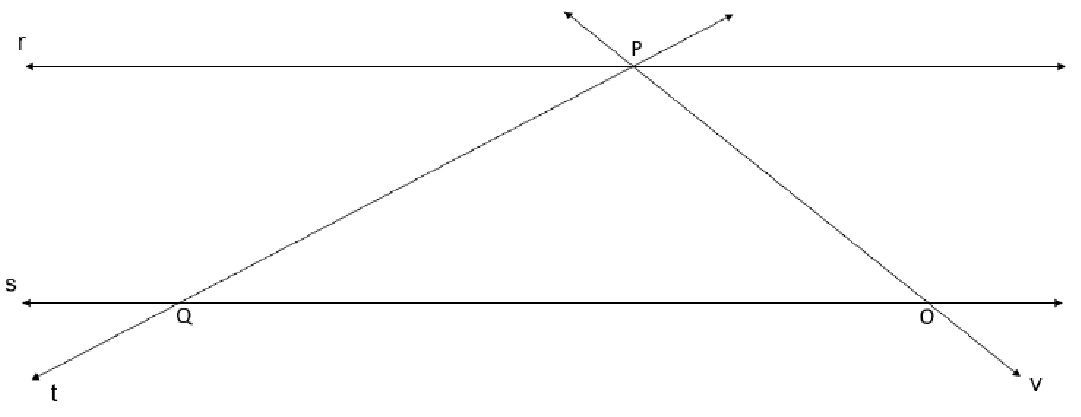
\includegraphics[width=0.95\linewidth]{static/simulados/coluni/latex-figs/2024-Q19.png}\end{center}

É CORRETO afirmar que o perímetro do triângulo $PQO$ mede, em cm:

\begin{enumerate}
	\item $21+\pi$
	\item $14\cdot(1+\pi)$
	\item $7\cdot(3+\pi)$
	\item $2\cdot(7+\pi)$
\end{enumerate}
